\section{Approach to Discover the Organizational Perspective}\label{sec:concept}

%Commit messages contain metadata and content. For analysis of users and roles both parts are important. Metadata includes the author, which is essential for gaining a unique identifier of the committer. The content gives some indications on roles. Data needs to be cleaned. Changed roles, one time committers, or several identities for the same use, are some of the challenges that need to be handled. 

Commits contain fine grained information about many aspects of a work unit. We are interested in three aspects. First we consider distinct identities and timestamps of commits. This makes it possible to compute how frequent and how distant in time commits appear in a project. Second, we obtain information about the authors. Authors are explicitly stated in the commit. Third, we consider their comments. Comments are written in natural language and need to be parsed and preprocessed before we can use them.

Once data is preprocessed, the analysis can start with a direct approach of connecting one commit message to one user and to the corresponding role. In this approach user roles are linked to the authors of commits. However, roles are not always available a priori. In these cases, a commit-based approach can be adopted. This method operates on the commits and assigns types to them first. Further analysis then maps these types to possible user roles. This approach is not a direct mapping. Instead, it allows for more flexible role discovery. We use this approach to also predict roles, based on user profiles that we create from the commit types.

\begin{figure}[htb]
   \centering
   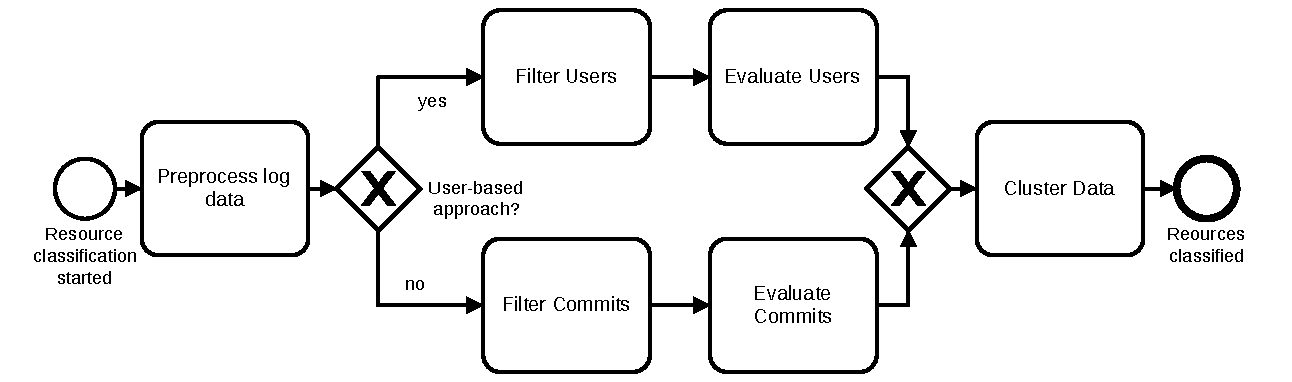
\includegraphics[width=1\linewidth]{ResourceClassification/figures/approach-bpmn}
   \caption[Approach to discover discover user roles from VCS logs]{Approach to discover discover user roles from VCS logs}
   \label{fig:approach-bpmn}
\end{figure}

\Cref{fig:approach-bpmn} illustrates the steps of our approach through a BPMN diagram. In the first step we preprocess the data and parse the SVN log file. Then we account for two different types of classification: user-based and commit-based. These approaches require a prior step where we filter the data according to users or to commits. Both approaches include an evaluation step where we map keywords and information on file types to users or commits, respectively. The last step is the data classification. \Cref{sec:impl} describes both approaches in detail.
